% -----------------------------------------------
% Template for ISMIR Papers
% 2025 version, based on previous ISMIR templates

% Requirements :
% * 6+n page length maximum
% * 10MB maximum file size
% * Copyright note must appear in the bottom left corner of first page
% * Clearer statement about citing own work in anonymized submission
% (see conference website for additional details)
% -----------------------------------------------

\documentclass{article}
\usepackage[T1]{fontenc}
\usepackage[utf8]{inputenc}
\usepackage[submission]{ismir} % Remove the "submission" option for camera-ready version
\usepackage{amsmath,cite,url}
\usepackage{graphicx}
\usepackage{color}
\usepackage{booktabs}
\usepackage{placeins}
\usepackage{amssymb}% http://ctan.org/pkg/amssymb
\usepackage{pifont}% http://ctan.org/pkg/pifont

\usepackage{cleveref} % Added for mutliple footnote
\crefformat{footnote}{#2\footnotemark[#1]#3}

\usepackage{algorithm} % Added
\usepackage{algpseudocode} % Added
\usepackage{gensymb} % Added
\usepackage{siunitx} % Added
\usepackage{multirow} % Added
\usepackage{kotex}
\newcommand{\cmark}{\ding{51}}%
\newcommand{\xmark}{\ding{55}}%

% Title. Please use IEEE-compliant title case when specifying the title here,
% as it has implications for the copyright notice
% ------
\title{PianoVAM: A Multimodal Piano Performance Dataset}
% 타이틀 정하기가 가장 어려운 것 같아요... (용현) ㅋ(준형) 인정합니다(기락) 

% Note: Please do NOT use \thanks or a \footnote in any of the author markup

% Single address
% To use with only one author or several with the same address
% ---------------
\oneauthor
  {Anonymous Authors}
  {Anonymous Affiliations\\\texttt{anonymous@ismir.net}}

% Two addresses
% --------------
%\twoauthors
%   {First author} {School \\ Department}
%   {Second author} {Company \\ Address}

% Three addresses
% --------------
% \threeauthors
%   {First Author} {Affiliation 1 \\ \texttt{author1@ismir.edu}}
%   {Second Author} {Affiliation 2 \\ \texttt{author2@ismir.edu}}
%   {Third Author} {Affiliation 3 \\ \texttt{author3@ismir.edu}}

% Four or more addresses
% OR alternative format for large number of co-authors
% ------------
% \multauthor
%   {First author$^1$ \hspace{1cm} Second author$^1$ \hspace{1cm} Third author$^2$}
%   {{\bf Fourth author$^3$ \hspace{1cm} Fifth author$^2$ \hspace{1cm} Sixth author$^1$}\\
%   $^1$ Department of Computer Science, University, Country\\
%   $^2$ International Laboratories, City, Country\\
%   $^3$ Company, Address\\
%   {\tt\small CorrespondenceAuthor@ismir.edu, PossibleOtherAuthor@ismir.edu}
%   }

% For the author list in the Creative Common license, please enter author names.
% Please abbreviate the first names of authors and add 'and' between the second to last and last authors.
\def\authorname{F. Author, S. Author, T. Author, F. Author, F. Author, S. Author and S. Author}

% Optional: To use hyperref, uncomment the following.
% \usepackage[bookmarks=false,pdfauthor={\authorname},pdfsubject={\pdfsubject},hidelinks]{hyperref}
% Mind the bookmarks=false option; bookmarks are incompatible with ismir.sty.

\sloppy % please retain sloppy command for improved formatting

\begin{document}

\maketitle

\begin{abstract}
% The intersection of music performance research and machine learning has heightened the need for multimodal datasets that combine audio, video, and symbolic data. We present PianoVAM, a comprehensive dataset featuring top-view performance videos, high-quality synchronized audio, MIDI data, and rich metadata including fingering labels. Designed for tasks such as piano transcription, performance analysis, score following, and multimodal music generation, PianoVAM offers precisely aligned multimodal data to support diverse research needs. We outline our data collection and preprocessing pipeline, addressing key synchronization challenges. Potential applications include automatic piano transcription, fingering detection, score following, performance analysis, and cross-modal learning. By releasing PianoVAM publicly, we aim to inspire advancements in computational musicology, MIR, and AI-driven performance modeling.

The convergence of music performance research and machine learning has created a growing demand for multimodal datasets that integrate audio, video, and symbolic data. This paper presents PianoVAM, a comprehensive dataset featuring synchronized top-view performance videos, audio, MIDI, and rich metadata. The metadata includes piece and performer information and keyboard corner coordinates. Additionally, the dataset incorporates fingering labels primarily generated by a MediaPipe-based heuristic algorithm, with human annotations added for undetected cases. We present the challenges encountered during data collection and the alignment process across different modalities. 
%This paper outlines the challenges encountered during data collection and preprocessing, along with the solutions devised.
By benchmarking PianoVAM's performance in piano transcription and fingering detection against established datasets and highlighting the unique benefits of incorporating video data, we demonstrate its potential to advance these tasks. Furthermore, we explore its broader utility in research areas such as crossmodal learning and performance analysis. 
\end{abstract}

\section{Introduction}\label{sec:introduction}
Music performance is inherently multimodal, extending beyond the auditory domain. Visual elements such as a musician's gestures, posture, and facial expressions significantly contribute to the communication of musical intent and emotional expressivity \cite{ISMIR24Choi, MP07Dahl, PsychMusic09Broughton, Thompson2005}. These visual cues play a critical role in audience perception and performance evaluation, sometimes even surpassing auditory information \cite{Moura2023, Tsay2013}. This underscores the importance of non-verbal expressivity in shaping how performances are perceived and appreciated.

Beyond audience perception, visual information can enhance key Music Information Retrieval (MIR) tasks, such as Automatic Music Transcription (AMT) and fingering estimation. 

AMT, which converts audio recordings into symbolic representations like MIDI or sheet music, has achieved significant progress through deep learning \cite{ISMIR18Hawthorne, TASLP21Kong, TASLP24Kwon}. However, audio-only transcription systems remain vulnerable in challenging acoustic conditions, such as noisy environments \cite{ISMIR24Kim}. While data augmentation techniques \cite{ISMIR24Kim, Edwards2024, ICLR19Hawthorne} have improved robustness, integrating visual data from performance videos has been shown to further enhance onset prediction \cite{CJE15Wan, ICASSPW23Li, TASLP24Li}. Visual cues such as hand movements and keyboard interactions provide additional context that audio alone may not fully capture.

Fingering information is widely recognized as a crucial aspect of piano performance, influencing both technical execution and expressive interpretation \cite{Piano21Telles}. Traditional methods for fingering estimation primarily rely on audio or (and) symbolic data \cite{IEAAIE10Maezawa, InfoSci20Nakamura, MM22Ramoneda}, which may produce inconsistent results due to variability in training data. Performance videos offer a valuable alternative by providing direct visual evidence of finger placement and movement \cite{MM07Zhang}. Despite this advantage, video-based fingering detection remains underexplored due to the scarcity of datasets that combine synchronized audio, video, symbolic notation, and explicit fingering annotations.

\FloatBarrier
\begin{table*}[htbp]
    \centering
    \caption{Comparison of Selected Piano Performance Datasets}
    \small
    \begin{tabular}{lcccccc}
        \toprule
        \textbf{Dataset}  & \textbf{Size (hrs)} & \textbf{Video} & \textbf{Audio} & \textbf{Audio Type} & \textbf{MIDI} & \textbf{Metadata} \\
        \midrule
        MAESTROv3 \cite{ICLR19Hawthorne}  & 198.7  & \xmark  & 44.1\si{kHz}, Stereo & Real  & \cmark & \cmark \\
        MAPS (MUS subset) \cite{Emiya2010}     & $\sim$18?  & \xmark     & 44\si{kHz}, Stereo & Synthesized \& Real & \cmark & \cmark \\
        OMAPS2 \cite{ICASSPW23Li}   & 6.7  & 1080p/30fps & 44.1\si{kHz}, Mono & Real & $\triangle$ (Restricted)  & \xmark \\
        PianoYT \cite{ICASSP20Koepke}  & $\sim$20  & Varies  & Varies? & Varies (YouTube) & $\triangle$ (Pseudo) & \cmark \\
        PIAST \cite{NLP4MusA24Bang} & $\sim$1006 & \xmark & Varies? & Varies (YouTube) & $\triangle$ (Pseudo) & \cmark \\
        PianoMotion10M \cite{ICLR24Gan} & $\sim$116 & \xmark & Varies? & Varies (Bilibili) & $\triangle$ (Pseudo) & \cmark \\
        PianoVAM (Ours) & 21.0 & 1080p/60fps & 44.1\si{kHz}, Mono & Real  & \cmark & \cmark \\
        \bottomrule
    \end{tabular}
    \label{tab:piano_datasets}
\end{table*}


Existing piano performance datasets typically address isolated or limited modalities (see Table \ref{tab:piano_datasets}). For instance, MAESTRO \cite{ICLR19Hawthorne} includes high-quality audio and MIDI data but lacks video recordings. MAPS \cite{Emiya2010} offers audio and MIDI from real performances (MUS subset), but a significant portion (210 out of 270 recordings) is synthesized rather than real audio. Datasets such as OMAPS2 \cite{ICASSPW23Li} and PianoYT \cite{ICASSP20Koepke} incorporate video data but provide limited MIDI annotations—OMAPS2 includes MIDI-like labels, while PianoYT relies on pseudo-MIDI annotations transcribed using the Onsets and Frames model \cite{ISMIR18Hawthorne}. Similarly, large-scale collections like PIAST \cite{NLP4MusA24Bang} provides extensive audio data and metadata but rely on pseudo-MIDI annotations transcribed via \cite{TASLP21Kong} and lack video content. 

To address these limitations, we introduce \textbf{PianoVAM}, a comprehensive 21-hour Video-Audio-MIDI dataset designed explicitly to support diverse applications in piano performance. PianoVAM features synchronized top-view performance videos, audio, MIDI data, and rich metadata, including fingering labels obtained primarily via our suggested rule-based algorithm based on MediaPipe, complemented by human annotations.

PianoVAM enables diverse research applications, including AMT, score-following and accompaniment systems, performance expression analysis, performer identification and style analysis, and multimodal learning and music generation. We briefly list these areas here and elaborate further in Section 
\ref{sec:fingering_detection}, \ref{sec:transcription} and
\ref{sec:future-rsearch-directions}.

This paper details the data collection and preprocessing procedures, presents an in-depth analysis of the dataset, and demonstrates PianoVAM's potential through case studies in transcription and fingering detection. We benchmark its performance against established datasets and highlight the benefits of incorporating video data. By publicly releasing PianoVAM, we aim to encourage research at the intersection of piano performance, machine learning, and multimodal signal processing.

\section{Dataset}\label{sec:dataset}
PianoVAM is available for download from the GitHub website\footnote{anonymized github link\label{github-link}} or Hugging Face\footnote{anonymized huggingface link}. A small subset of the dataset and data loader are also provided for convenience.

% 피아노 채보 성능 (처음 마주하는 곡 / 처음 마주하는 연주자)

\subsection{Acquisition}
Acquiring synchronized piano performance video, audio, and MIDI is challenging, particularly in achieving precise alignment across modalities. Efficient metadata collection, such as piece details and performer information, is best integrated into the acquisition process but should remain unobtrusive to both performers and annotators. To address these challenges, we developed PiaRec, a dedicated system designed to optimize user experience and streamline data collection. PiaRec enables performers to contribute data independently, without external assistance, while automating post-processing to achieve approximate synchronization between audio and video, minimizing manual effort.

\subsubsection{PiaRec Workflow}
The PiaRec workflow comprises the following steps:

\textbf{User Registration:} First-time users are required to complete a registration process that collects key performer information, including self-assessed proficiency (categorized into three levels: Beginner, Intermediate, Advanced), age group, and gender. Upon successful registration, users receive an email containing three QR codes: one associated with their profile and two for system control, serving as triggers to start and stop recording. 

\textbf{System Initialization:} The recording environment is activated by clicking the PiaRec launch button, integrated with StreamDeck for convenience. This action initializes the PiaRec main interface, OBS Studio for video and audio recording, and Logic Pro for audio and MIDI recording, all displayed on the PC screen.

\textbf{Recording Setup:} Before each session, users enter performance-specific details in the Record tab. All required fields must be completed before proceeding.

\textbf{Recording Process:} After confirming performance details, users display their profile QR code to the top-view camera. PiaRec then activates the previously initialized recording software (OBS Studio and Logic Pro).

\textbf{Stopping the Recording:} During the performance, the system continuously monitors for QR code events. Displaying the stop QR code prompts PiaRec to halt all recordings. PiaRec then aligns the tracks by comparing the first 10 seconds of each recorded audio file, trimming the earlier track to ensure proper synchronization.

\subsubsection{Hardware Setup for PiaRec}
The PiaRec system's hardware setup includes a PC running the PiaRec Python script alongside OBS Studio and Logic Pro. OBS Studio records video and audio, while Logic Pro captures audio and MIDI data. Recording audio in both applications enables rough synchronization of video and MIDI using cross-correlation between the two audio tracks. An automated piano (Disklavier) captures MIDI data, while a microphone records audio. A webcam with appropriate mounting equipment provides top-view video footage of performances. Optionally, a StreamDeck can be integrated to simplify system initialization.

\begin{figure}
    \centering
    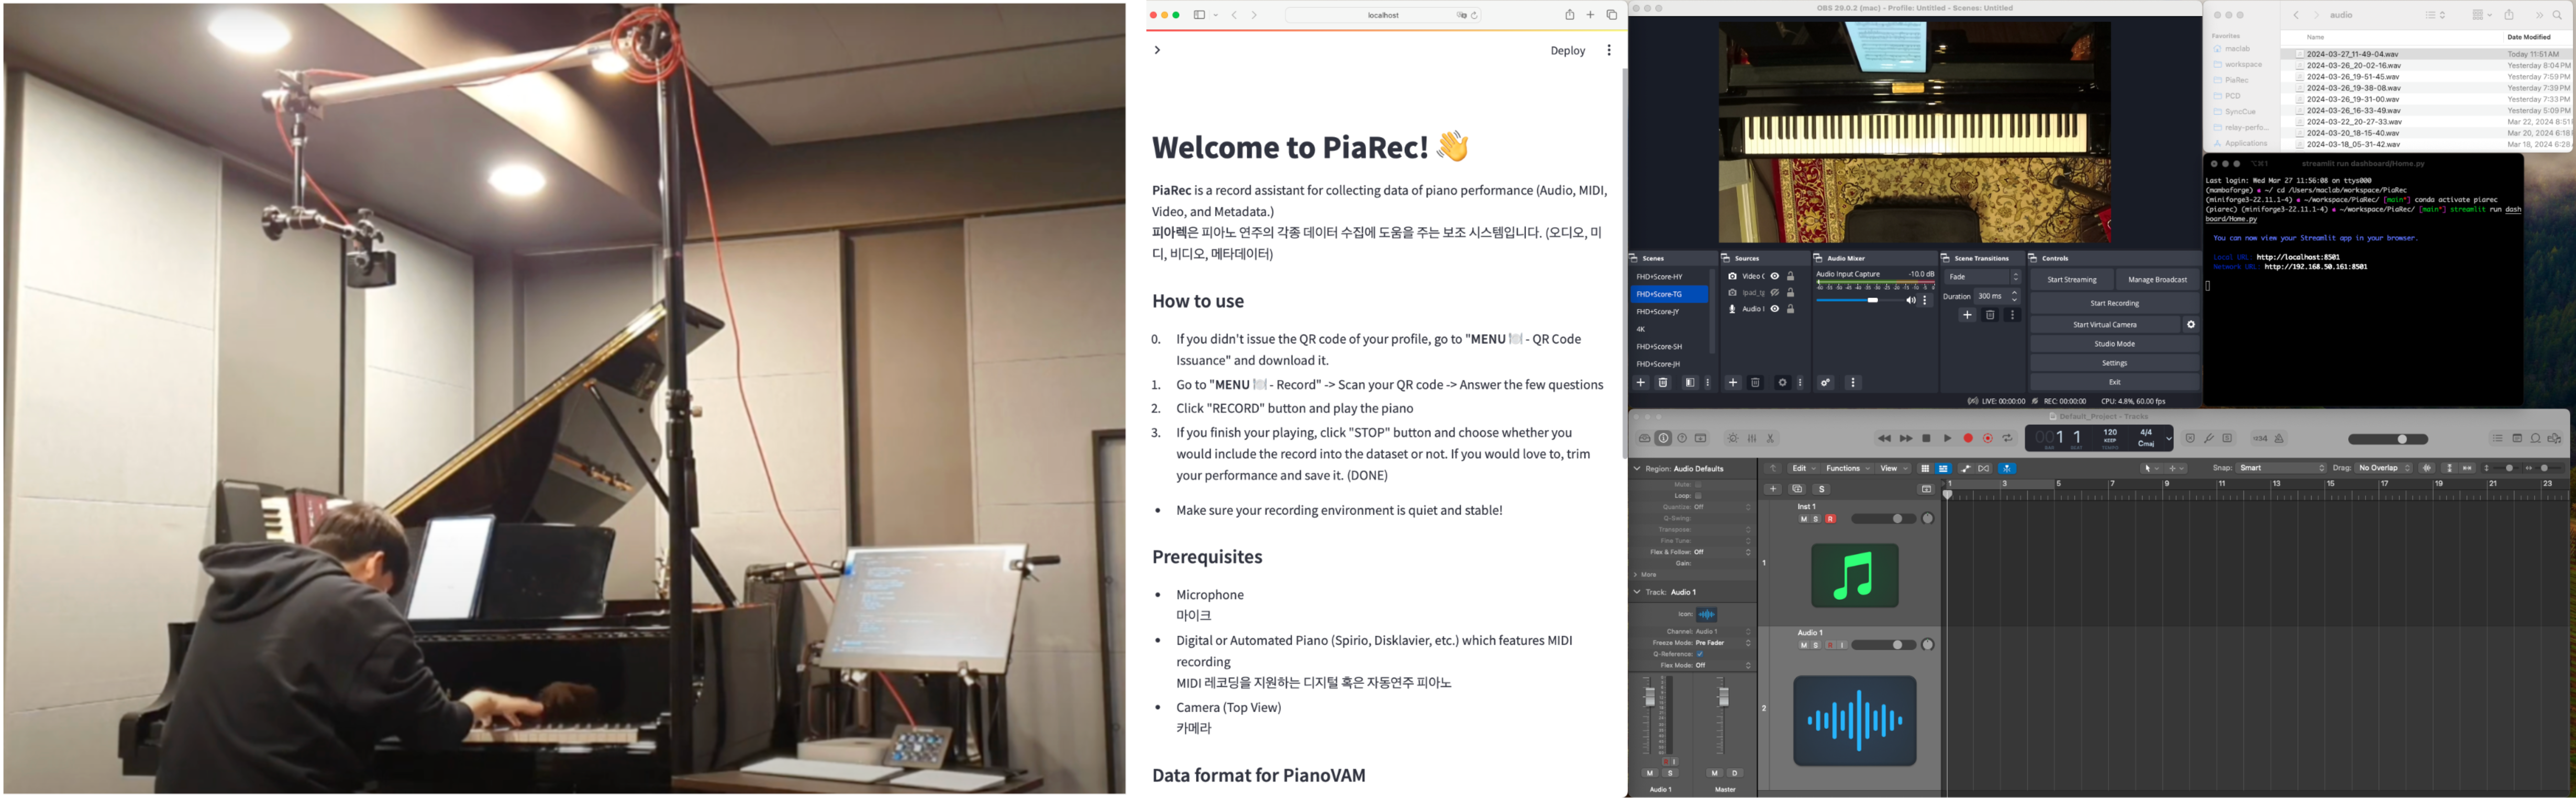
\includegraphics[width=\linewidth]{Images/PiaRec.png}\hspace*{0cm}
    \caption{Caption}
    \label{fig:piarec}
\end{figure}

% 하드웨어 및 소프트웨어 셋업 등 자세히 기입
% 오디오, 비디오, 미디, 메타데이터가 어떻게 수집되었는지 상세히 기입

\begin{figure}
    \centering
    \includegraphics[width=\linewidth]{Images/performer_composer_distribution.pdf}\hspace*{0cm}
    \caption{Caption}
    \label{fig:performer_composer_distribution}
\end{figure}

\subsection{Preprocessing}
\subsubsection{Alignment}
%https://docs.google.com/document/d/1G1aIxIEiFI9kxwOgP_GDq4pADkeToc136394PAb-5-I/edit?usp=sharing
Roughly aligned audio and MIDI data were further refined using the fine alignment strategy proposed in the MAESTRO paper \cite{hawthorne2019enablingfactorizedpianomusic}. While they employ both coarse and fine alignment steps to address significant misalignment and residual jitter, only the fine alignment step was applied in this study, as no major misalignment was observed. Both audio and MIDI data were resampled to 22,050\si{Hz} mono, and a Constant-Q Transform (CQT) was extracted with a hop length of 64 ($\sim$3\si{ms} resolution). Dynamic Time Warping (DTW) was then applied within a Sakoe-Chiba band of ±2.5\si{s} to correct any remaining temporal discrepancies, such as residual jitter or constant offsets.

\subsubsection{Audio Loudness Normalization}
While piano transcription models are generally designed to predict MIDI velocity independently of audio loudness, a correlation between the two is difficult to ignore \cite{}. In our dataset, recordings were collected over a period exceeding six months in a shared studio, often without additional assistance during data collection. This led to variability in loudness levels, likely due to inconsistent audio interface gain settings. To ensure consistent loudness-velocity relationships across the dataset, we applied a loudness normalization procedure. First, the collected MIDI data were synthesized using \textit{FluidSynth} with a Disklavier-sampled SoundFont (YDP Grand Piano SoundFont, Version 2016-08-04) \footnote{https://freepats.zenvoid.org/Piano/acoustic-grand-piano.html}. The loudness of the rendered audio was then measured using the \textit{pyloudnorm} package. Finally, the dataset's overall average loudness was standardized to -23 LUFS. This process improved loudness-velocity consistency while preserving the natural dynamic range of the performances.

\subsubsection{Data Splitting}
To facilitate comparison with our results, we recommend utilizing the provided data splits, designed to meet the following criteria: (1) no composition appears in more than one split, and (2) the dataset is divided approximately into 80/10/10 percent for the training, validation, and test sets, respectively, based on total duration. A unique 4-hands performance (2024-02-15\_22-12-41) was assigned to the test set, as it may present a special case for deep learning models that incorporate video inputs. Consequently, the train/validation/test sets contain 73, 19, and 15 files, respectively. While these splits are intended to support consistent comparison with our results, we encourage future researchers to adapt the data split strategy as needed to suit their specific experimental objectives.

\subsection{Statistics}
% Working on
The dataset comprises 107 recordings spanning approximately 21 hours, featuring 10 unique amateur performers and 38 composers.(Figure \ref{fig:performer_composer_distribution})  With the exception of one 4-hands performance, all recordings are solo performances. Among the solo performers, self-reported skill levels are distributed across 70 advanced, 26 intermediate, and 10 beginner. Pedaling Distribution (Figure \ref{fig:Pedal-Comparison})

\begin{figure}
    \centering
    \includegraphics[width=\linewidth]{Images/pedal_comparison.pdf}\hspace*{0cm}
    \caption{Distribution of file-level pedal usage ratios in MAESTROv3 and PianoVAM datasets.}
    \label{fig:Pedal-Comparison}
\end{figure}

% 총 몇명의 연주자가 플레이했고 몇명의 작곡가가 있었으며, 각 연주자별 / 작곡가별 데이터셋에 차지하는 비율을 위아래로 subplot으로 그리기

% The dataset includes 91 male and 16 female performances, with most being solo performances (106) and one 4-hands performance (Intermediate + Advanced).

% Table

\section{Fingering Detection}\label{sec:fingering_detection}
% 준형 알고리즘 소개
% Brief Introduction to the Algorithm can be input here (Yonghyun)

The dataset includes both audio and video data, enabling a variety of derivative research opportunities. Leveraging MediaPipe Hands\cite{arXiv20Zhang}, one of the state-of-the-art hand landmark detectors, we developed an algorithm that automatically detects fingering annotations by extracting skeletal hand coordinates from the dataset. This algorithm achieves a precision of 95\%. However, due to performance limitations caused by complex playing techniques or ambiguous fingering positions, it has a detection miss rate of approximately 20\%. To address these gaps, we developed an efficient fingering labeling GUI\cref{github-link} to supplement the annotations.

%We provide a GUI on GitHub to easily point out corner location information and lens distortion coefficient.

% The first draft of the Fingering Detection was written by Junhyung, and I (Yonghyun) will look, and try to revise the phrasing as soon as possible. 
\subsection{Inputs \& Outputs}
The inputs are video files and MIDI files in the PianoVAM dataset synced within 5 ms, the locations of the four corners of the piano keyboard, and lens distortion coefficients in the first frame for each video, which can also be set manually by the GUI. Note that the data need few preprocedures, so that our algorithm could be applied to other multimodal datasets.
The outputs are fingering information and a separated MIDI file by each hand.

%아니면 다른 데이터셋에서도 활용할 수 있다는 걸 강조하기 위해서 그냥 video and midi synced in 5ms 정도로만 적어도 괜찮을까 싶네요. (Junhyung)

\begin{table*}[htbp]
    \centering
    \caption{Comparison of Piano Fingering Datasets}
    \small
    \begin{tabular}{lcccccc}
        \toprule
        \textbf{Dataset}  & \textbf{Size (hrs)} & \textbf{\# of pieces} & \textbf{Labeled ratio} & \textbf{Precision?} & \textbf{Extendability} \\
        \midrule
        PIG \cite{InfoSci20Nakamura} & $\sim$? & 150 & 100\% & 1 & \xmark \\
        Thumbset \cite{} & ? & 2523 & 52\%  & ? (Labeled by miscellenous) & \xmark \\
        PianoVAM-Finger (Ours) & ? & ? & 80\% (+20\% by human) & 0.95 & \cmark \\
        \bottomrule
    \end{tabular}
    \label{tab:alrogithm}
\end{table*}

\subsection{Algorithm}
% 
Our algorithm suggests candidates of fingers that are likely to play each note in the MIDI file, by utilizing \cite{arXiv20Zhang} to detect hand landmark information from input video.
\begin{figure}
    \centering
    \includegraphics[width=\linewidth]{fingeringdetection.png}\hspace*{0cm}
    \caption{Process diagram of fingering detection algorithm}
    \label{fig:enter-label}
\end{figure}

At first, we detect floating hands framewise, which obviously do not play any notes, to handle hand-crossing. We define a metric to measure the $z$-depth of hand. For each video, we find the \textit{model skeleton} of each hand, then calculate the z-axis of each hand from the model skeleton. The model skeleton should be unbent, not tilted, and on the keyboard. For tiltedness, the plane decided by three hand keypoints, namely Wrist ($W$), Index Finger Metacarpals ($I$) and Ring Finger Metacarpals ($R$), should be parallel to the plane of the keyboard. We assume that the angle $\angle IWR$ is kept almost $28\degree$, which is a heuristic estimate for the average human hand in its neutral position (citation pending; finger abduction angle ~ adduction angle?), in the situation where the hand is not bent and not tilted. To measure how much the hand is bent, we calculate the ratio $r=\frac{|\triangle WIR|}{|WF_{1}F_{2}F_{3}F_{4}F_{5}|}$ of $|\triangle WIR|$ and area of the hexagon $|WF_{1}F_{2}F_{3}F_{4}F_{5}|$ where $F_i$ is the fingertip of the $i$th finger. Finally, to take the hand which is on the keyboard, we simply select the median by the area of $\triangle WIR$. So we can select the model hand as
\begin{equation}
    W_{0}I_{0}R_{0}=\underset{|\angle IWR - 28\degree| \text{ low 10\%}, r \text{ high 50\%}}{\text{median}}|\triangle IWR|
\end{equation}
Let the plane of projected 2D image be $z=z_{0}$, and the area of 2D image be
\begin{equation}
  \begin{aligned}
    A:=\{(x,y)  | x\in (-1,1), y\in (-r,r)\} \subset \mathbb{R}^2
    \\\cong\{(x,y,z_{0})|x\in(-1,1), y\in (-r,r)\}\subset \mathbf{P}\mathbb{R}^3
\end{aligned}  
\end{equation}
where the origin of real projective space $\mathbf{P}\mathbb{R}^3$ is the center of the lens of the camera and $r$ is the ratio of video resolution. Our goal is to calculate the relative depth rather than the real depth, so we let $z_{0}=1$ for convenience of calculation. \\
Now, we are ready to calculate the relative $z$-depth of the hands. Knowing from the fact that the original point is contained in the line $\{(xt,yt,t) | t\in \mathbb{R^{+}}\}$, we have three equations and three variables: Solve $t,u,v>0$ from
\begin{gather}
    \left||(x_{W}t,y_{W}t,t),(x_{I}u,y_{I}u,u)|\right|_{\mathbb{R}^3}=\left|\overline{W_{0}I_{0}}\right| \\
    \left||(x_{I}u,y_{I}u,u),(x_{R}v,y_{R}v,v)|\right|_{\mathbb{R}^3}=\left|\overline{I_{0}R_{0}}\right| \\
    \left||(x_{R}v,y_{R}v,v),(x_{W}t,y_{W}t,t)|\right|_{\mathbb{R}^3}=\left|\overline{R_{0}W_{0}}\right|.
\end{gather}
Note that if three elliptical cylinders are in general position, there must exist a solution. Also, the number of solutions is at most 4 by B\'{e}zout's theorem and symmetry. Here, our desired solution can be approximately calculated using Powell's dog leg algorithm with a close initial guess $(t,u,v)=(1,1,1)$.
Finally, $d=\displaystyle\frac{t+u+v}{3}$ becomes the $z$-depth of mass of the center of the hand skeleton of each frame. From (3)$\sim$(5), it is obvious that $d_{\text{model}}=1$ for each hand.\\
Now, we decide that the targeted hand of targeted frame is floating if (6) holds: 
\begin{equation}
    \frac{1}{2}\mathbf{d}_{\pm k\text{frames}} \cdot \frac{1}{k(k-2)}[1,2,\cdots, k,\cdots, 1]+\frac{1}{2}d_{\text{frame}}<0.9
\end{equation} where $\mathbf{d}_{\pm kframes}$ is vector of depths of $2k-1$ frames near the target frame, and if there are some frames inavailable to detect targeted hand with MediaPipe, instead we just use depth of the targeted frame. In (6), we consider the depth of close frames as hand motion is continuous. Empirically, we involved 0.25 seconds of finger motion to the finger score, in other words, $k=7$.\\
\begin{algorithm}[h]
\caption{Fingering Candidate Selection Algorithm}\label{alg:cap}
\begin{algorithmic}
\State $N = \text{Total number of notes}$
\State $K(n) = \text{Keyboard area of $n$th note}$
\State $R(n) = \text{Range of frames of $n$th note played}$
\State $H(f,i) = i\text{th Finger location info of frame $f$,} $ but fingers of floating hands are not contained
\State $w = \text{width of a key}$ 
\For{$n < N$}
\State $S_n \gets (0,0,\cdots, 0)$ \Comment{Score of each finger likely playing $n$th note}
\For{$f \in R(n)$}
\For{$i<10$}
\If{\text{each }$H(f,i) \in K(n)$}
\State $S_n\gets S_n + \chi_i$ \Comment{$\chi_i$ = $i$th unit vector}
\ElsIf{$0<||H(f,i),K(n)||_{\mathbb{R}^2}< w$}
\State $S_n \gets S_n + \left(\frac{1-||H(f,i),K(n)||_{\mathbb{R}^2}}{w}\right)^{2}$
\EndIf
\EndFor
\EndFor
\EndFor
\For{$n<N$}
\If{$\exists i \ s.t. \ S_n \cdot \chi_i > 0.5|R(n)|$}
\If{$\exists ! \ i$}
\State $i$ is the only candidate
\ElsIf{$\exists ! \ i \ s.t. \ S_n \cdot \chi_i > 0.8|R(n)|$}
\State $i$ is the only candidate
\Else \text{ }  There are multiple candidates
\EndIf
\Else \text{ } There are no candidates
\EndIf
\EndFor
\end{algorithmic}
\end{algorithm}
After detecting all floating hands, we can choose possible candidates for the fingering by using Algorithm 1. We calculate the finger score for each note by the number of frames in which the fingertip is in the selected note area. If the fingertip is slightly off from the area in some frames, we add the correction value that is less than a frame whose fingertip is totally in the keyboard area. From the score of each finger of the $n$th note, we add the finger as a candidate or a strong candidate if the score is greater than 50\% or 80\% of the length of the note, respectively. If there exist multiple candidates, but a unique strong candidate, we leave the strong candidate as the only candidate. Note that there can be some notes with no candidate or multiple candidates, hence our algorithm can leave few notes unlabeled.

\subsection{Results}
In Table \ref{tab:fingering_results}, we calculated the precision for the first 150 notes of 10 different data in PianoVAM with the groundtruth fingering labeled manually. Except for some specific case such as \textit{Chopin's Grande valse brilliante, Op.18}, the precision exceeds 95\%, and there were also few unlabeled notes, whose ratio is approximately under 10\%.
\begin{table}[htbp]
\centering
\small
\caption{Results of fingering detection over first 150 notes of 7 pieces}
\label{tab:fingering_results}
\begin{center}
\begin{tabular}{c c c c}
\toprule
\multirow{2}{*}{\textbf{Piece name}} &  \textbf{Precision} & \textbf{Multi}  & \textbf{No} \\                                         &  \textbf{(First 150)} & \textbf{Candi.} & \textbf{Candi.}\\
\midrule
Chopin, Op.18 & 76.5\% & 11\% & 5\% \\
Debussy, L.75 Mvt.3 & & & \\
Grieg, Op.16 Mvt.2 & & & \\
Yiruma, Kiss the Rain 99\% & 7\% & 3\% & \\
Improvisation & & & \\
Schumann, Op.17 Mvt.1 & & & \\
Kapustin, Op.40 No.6 99\% & 10\% & 3\% & \\
Ver.2 Data 1 & & & \\
Ver.2 Data 2 & & & \\
Ver.2 Data 3 & & & \\
\midrule
\end{tabular}
\end{center}
\end{table}
Compared to other fingering datasets such as PIG\cite{} and Thumbset\cite{}, our algorithm provides the opportunity to make a large-scale fingering dataset by applying our algorithm to other datasets that have MIDI data synced with top-view videos. In particular, we expect high-quality fingering from datasets with more advanced performers. \\ 
Chopin's waltz contains fast note repetition, which makes several fingers above the note to prepare to play that repeated note. In this situation, our algorithm can make false decisions since several fingers are in the note area and in full note length, since the note length is very short, which is about 2 or 3 frames. False decisions also occur from MediaPipe errors, due to blurry frame images, head interruption, or sleeve interruption. We expect that using newer hand pose estimation models such as ViTPose+ \cite{} can lead to higher precision.

%PIG dataset, Thumbset dataset 비교
%Hyperparameter justification 

\section{Automatic Piano Transcription}\label{sec:transcription}
Automatic Music Transcription (AMT) is a key research area in Music Information Retrieval (MIR), particularly for piano transcription. While AMT systems have traditionally relied on audio as the primary input, recent studies have explored the use of video data.

Koepke et al. \cite{Koepke} introduced Visual Music Transcription (VMT), which leverages video to predict note onsets. Other approaches incorporate visual information in post-processing to refine onset predictions in audio-only AMT systems. Additionally, a two-stage method trains audio and video modules separately and then fuses their features for onset prediction. These efforts highlight the potential of visual data in music analysis.

\subsection{Audio-Only Piano Transcription}

To validate the effectiveness of our newly introduced dataset, PianoVAM, we conducted a comparative analysis with MAESTROv3, a commonly used dataset in piano transcription research. For this experiment, we reproduced the Onsets and Frames\cite{ISMIR18Hawthorne} following its original specifications and employed it for evaluation. The model was independently trained and evaluated on each dataset to assess their comparability. For evaluation, we utilized the model weights corresponding to the checkpoint with the lowest validation loss. All results in Table \ref{tab:performance_comparison} are presented as F1 Scores (\%) and calculated over the entire duration of the respective test splits. The terms Onset, w/ Offset, and w/ Vel. refer to Onset, Onset with Offset, and Onset with Velocity, respectively. All four evaluation metrics, including Frame, were computed using the \textit{mir\_eval} package. In accordance with established conventions in transcription research, Offset timings were adjusted to the pedal-release time if the sustain pedal remained engaged.
% Onset tolerance: 0.05, minimum offset tolerance: 0.05, offset ratio: 0.2 (477 line of https://github.com/mir-evaluation/mir_eval/blob/main/mir_eval/transcription.py)
\begin{table}[htbp]
\centering
\small
\caption{F1 Score Comparison of Models Trained on Different Datasets (MAE3: MAESTROv3, PVAM: PianoVAM, Mixed: MAE3 + PVAM)}
\label{tab:performance_comparison}
\begin{tabular}{l l c c c c}
\toprule
\textbf{Train} & \textbf{Test} & \textbf{Onset} & \textbf{w/ Offset} & \textbf{w/ Vel.} & \textbf{Frame} \\
\midrule
\multirow{2}{*}{MAE3} & MAE3 & 94.2 & 76.5 & 92.3 & 87.1 \\
                           & PVAM   & 92.9 & 61.4 & 89.6 & 77.8 \\
\midrule
\multirow{2}{*}{PVAM}  & MAE3  & 83.1 & 5.0   & 64.6   & 30.6   \\
                           & PVAM   & 95.5 & 57.5 & 93.2 & 79.2 \\
\midrule
\multirow{2}{*}{Mixed} & MAE3  & 94.2 & 75.8 & 92.2  & 86.0 \\
                           & PVAM   & 94.9 & 70.9 & 92.5 & 86.3 \\
\bottomrule
\end{tabular}
\end{table}

% Test with MAPS?
% Currently Evaluating w/ Filtered MAE3 (Same File Number with similar pedaling usage w/ PVAM test split) [Model: Train on PVAM] --> Doesn't improve the performance. (79.7, 4.2, 60.8, 36.6)


% Working on
We trained our model using three distinct dataset configurations: MAESTROv3, PianoVAM, and Mixed (a combination of MAESTROv3 and PianoVAM). For testing, we utilized the model checkpoint corresponding to the lowest validation loss observed during training.

As commonly observed, performance degrades when there is a mismatch between the training and testing datasets, likely due to differences in recording environments, playing styles, or other factors. Notably, a significant performance gap was observed in Offset metrics between MAESTROv3 and PianoVAM. To investigate the impact of combined training data, we performed an additional experiment by merging all files from MAESTROv3 and PianoVAM into a single dataset. Despite the size imbalance between the two datasets, training on this combined dataset improved performance when evaluated on individual datasets. This suggests that exposing the model to diverse recording conditions during training can mitigate performance degradation on unfamiliar data.

% PianoVAM train split: 73 valid split: 19 (files)
% MAESTROv3 train split: 962 valid split: 137 (files)


% Possibility of the Pedal Usage?
% # MAESTRO: 61.69% (Pedal)
% # PianoVAM: 81.64% (Pedal)

% I will change the offset min tolerance (0.05 sec -> 0.10 sec) and check the result.
% tmux 11 Only min_tolerance
% tmux 12 w/ offset_ratio 0.2 -> 0.4
% Onset tolerance ->50 ms 
% Offset tolerance -> ? ms
% Offset ratio of 0.2,

% Possibility of the scarcity of the data amount? (I think so)
% For MAPS, Onsets and Frames shows 50.22 F1-Score for Note + Offset
% MAESTROv3: 198.7 hours
% PIANOVAM: 21.0 hours

% I will test again with other checkpoint (further trained)

% Try with same amount of data w/ MAESTRO and try again? -- Training data might not enought to learn the offset precisely. If 


% 지금 PianoVAM은 오프셋을 학습하는게 MAESTRO보다 어려워함 (페달이 누른 경우가 더 많은 것으로 짐작감) --> 빠르게 테스트하기 위해 PianoVAM에서 페달이 밟히지 않은 구간만 훈련으로 진행했을때를 비교해보면 될 것 같다. (우선 데이터셋간의 key_offset, frame_offset간의 미스매치율을 비교; PianoVAM이 MAESTRO보다 많은 것으로 짐작됨.) 

% \subsubsection{Video-Only Piano Transcriptoin}
% [Video-Only Model]
% Sight To Sound
% Train  \& Test by {OMAPS2, PianoVAM}

\subsection{Audio-Visual Piano Transcription}
% I will introduce my algorithm (Post-Processing) to showcase the advantage of the top-view video. (Ongoing)

Various approaches have been explored for piano transcription when both audio and video are available. For instance, \cite{CJE15Wan,} proposed a method that enhances the results of an Audio-Only AMT system by incorporating visual information, while \cite{,TASLP24Li} utilized both audio and video as inputs to improve onset prediction. In this work, we propose a pipeline that refines predicted MIDI notes from an Audio-Only AMT system by leveraging top-view video, piano keyboard corner coordinates, and the MediaPipe Hands\cite{arXiv20Zhang} to eliminate unreachable notes.

The pipeline begins by extracting onset information from the predicted MIDI. For each onset, the closest video frame is identified, and hand landmarks are predicted using MediaPipe. Each video frame's timestamp is defined as the midpoint of the time interval it covers. If both hands are undetected, the corresponding onset is skipped. For detected cases, the keyboard corner metadata is used to perform a perspective transformation, generating a rectangular image with dimensions 125×1024 — a size chosen to match the standard height-to-width ratio (1:8.147) of an 88-key piano. The predicted hand landmark coordinates undergo the same transformation. Assuming the 52 white keys are evenly spaced, the algorithm identifies the corresponding white key region for each fingertip's x-coordinate. To account for potential distortions caused by MediaPipe tracking or the keyboard's perspective, multiple candidate keys are accepted. The threshold for determining the number of candidates is treated as a hyperparameter. The intersection of candidate keys across all ten fingertips defines the final set of valid pitch candidates. For each onset, if the predicted pitch from the Audio-Only AMT system falls within the identified pitch candidates, the note is retained; otherwise, it is discarded. This procedure is applied iteratively to refine the transcription for all onsets. Detailed information and code are available on GitHub\cref{github-link}.


(Graph will be posted here.)
% or Graph (x-axis: Different Key candidates threshold; +- keys)

The proposed algorithm shows that Onset F1 increases after applying it to the Audio-Only AMT's predicted MIDI. Onset

Onset Precision gets increase with 

[Nature of Note Elimination]
Recall lower -> Eliminating the Answer
Higher Precision --> Eliminating the Wrong data

% [Audio-Visual Model]
% Post-Processing \& AVF
% Train \& Test by {OMAPS2, PianoVAM}

% Audio-Only, Video-Only, Audio-Visual


% Top view video aligned with MIDI인 다른 데이터셋이 있다면, 그 데이터셋으로부터 적은 인간 노력으로 평균 95% 이상 accuracy의 fingering dataset을 만드는 것이 가능하다. 특히, 연주자의 수준이 높은 데이터셋일수록 위의 algorithm으로부터 양질의 fingering dataset을 기대할 수 있다. 또한, further work로 ViTPose+와 같은 새로운 hand pose estimation 모델을 적용하여 더 높은 precision을 달성하는 것 또한 기대할 수 있다.


% PianoVAM's multimodal design opens opportunities for a wide range of research directions, including:

% \begin{itemize} 
% \item \textbf{Automatic Music Transcription}: 페달링정보가 포함된 미디는 pedal detection \cite{})과 더불어, Leveraging additional non-audio(visual, metadata) cues for improved transcription accuracy in real-world acoustics. 

% \item \textbf{Score-Following and Accompaniment Systems}: 피아노 채보와 마찬가지로 오디오를 인풋으로 하여 분석하는 스코어 팔로잉은 레코딩 상황에 있어 robust하게 작동함을 요구로한다. 이와 더불어 타연주자와의 합을 맞추는 AI 반주자 혹은 AI 콜라보 연주자를 제작하기 위해서는 큐 디텍션까지 고려를 해야하는데 오디오 만으로는 정확한 타이밍의 큐를 기대하기가 어렵다 \cite{}. 이러한 상황에서는 visual cues가 큰 도움을 줄 수 있다.

% \item \textbf{Performance Expression Analysis}: Examining how pianists convey expressivity through timing, articulation, and motion. 

% \item \textbf{Performer Identification and Style Analysis}: Investigating the relationship between movement patterns and individual performance styles. 

% \item \textbf{Multimodal Learning and Music Generation}: Training models to synthesize realistic performances conditioned on different modalities. 
% \end{itemize}
\section{Future Research Directions}
\label{sec:future-rsearch-directions}
% \subsection{Robust Piano Transcription}\label{subsec:robust_piano_transcription}
% Piano transcription is a prominent research area in Music Information Retrieval (MIR), with recent models achieving impressive results \cite{}. However, these models are typically evaluated on clean audio, and their performance often deteriorates in real-world conditions with noise and reverberation.

% Incorporating noise injection techniques during training has been shown to improve robustness in noisy environments \cite{ISMIR24Kim}, yet there remains room for further enhancement. Leveraging visual information alongside audio has proven effective in mitigating transcription errors, particularly harmonic ambiguities that are challenging to resolve from audio alone. Visual cues, such as the pianist's hand movements and interactions with the keyboard, provide valuable context that can further enhance model robustness in noisy conditions.

\subsection{Score-Following and Accompaniment Systems}\label{subsec:score_following}
Score-following systems analyze live audio input to track a musician's position in the score in real-time. These systems are crucial for robust performance synchronization in both live concerts and practice environments. However, score-following systems relying solely on audio often struggle under challenging recording conditions. Integrating visual cues, such as hand movements and keypress gestures, can improve robustness by providing additional context for score alignment. Similarly, developing AI-based accompaniment systems that collaborate with live performers requires precise cue detection to ensure timing accuracy. Visual information plays a key role in recognizing physical cues from the performer, such as hand gestures indicating tempo changes or performance intensity, which are difficult to capture from audio alone \cite{}.


\subsection{Performance Expression Analysis}\label{subsec:performance_expression}
Analyzing expressive elements in piano performance—such as timing, articulation, and dynamic control—can provide insights into a performer's interpretative choices. By combining audio, MIDI, and visual data, researchers can investigate how pianists convey expressivity through their movements, offering a deeper understanding of the interplay between physical gestures and musical phrasing.

\subsection{Performer Identification and Style Analysis}\label{subsec:performer_identification}
Although our dataset might be insufficient to conduct the following research, $\sim$.
Piano performance is highly individualized, with each performer exhibiting unique timing patterns, articulation preferences, and expressive gestures. By studying visual movement patterns alongside audio and symbolic data, researchers can analyze stylistic differences between performers, opening new possibilities for performer identification, style analysis, and expressive performance synthesis.

\subsection{Crossmodal Learning and Multimodal Generation}\label{subsec:crossmodal_learning}
The multimodal nature of PianoVAM presents new opportunities for crossmodal learning and multimodal generation tasks. While predicting MIDI data from performance audio is commonly known as automatic music transcription, deeper exploration of the relationship between audio and video enables additional tasks such as synthesizing expressive performance audio from visual data or generating synchronized performance videos from audio and MIDI. These capabilities open new pathways for performance visualization, music learning systems, and creative applications. By leveraging PianoVAM’s synchronized data streams, researchers can develop robust models that enhance transcription accuracy, improve performance analysis, and enable innovative crossmodal generation techniques.
\section{Discussion}\label{sec:discussion}
Still, More Data (Especially w/o Pedal cases) might be needed.

\section{Conclusion}\label{sec:conclusion}
% \section{Acknowledgments}

% You may include an optional Acknowledgments section in your camera-ready version to refer to any individuals or organizations that should be acknowledged in your paper. \textbf{Do not include the Acknowledgments section in your submitted manuscript.} The Acknowledgments section does \textit{not} count towards the page limit for scientific content.

\section{Ethics Statement}
% You may include an optional Ethics Statement section to provide additional ethical considerations related to your paper. The Ethics Statement section can be included both at submission time and in your camera-ready version. See the Call for Papers for details. The Ethics Statement section does \textit{not} count towards the page limit for scientific content.
This study involved human participants for data collection, which was approved by the Institutional Review Board (IRB) at \textit{anonymized} (Approval No. \textit{anonymized}). All procedures strictly adhered to established ethical guidelines to ensure the participants' rights, safety, and well-being.


% For BibTeX users:
\bibliography{ISMIRtemplate}

% For non BibTeX users:
%\begin{thebibliography}{citations}
% \bibitem{Author:17}
% E.~Author and B.~Authour, ``The title of the conference paper,'' in {\em Proc.
% of the Int. Society for Music Information Retrieval Conf.}, (Suzhou, China),
% pp.~111--117, 2017.
%
% \bibitem{Someone:10}
% A.~Someone, B.~Someone, and C.~Someone, ``The title of the journal paper,''
%  {\em Journal of New Music Research}, vol.~A, pp.~111--222, September 2010.
%
% \bibitem{Person:20}
% O.~Person, {\em Title of the Book}.
% \newblock Montr\'{e}al, Canada: McGill-Queen's University Press, 2021.
%
% \bibitem{Person:09}
% F.~Person and S.~Person, ``Title of a chapter this book,'' in {\em A Book
% Containing Delightful Chapters} (A.~G. Editor, ed.), pp.~58--102, Tokyo,
% Japan: The Publisher, 2009.
%
%\end{thebibliography}

\end{document}
